\documentclass[hyperref={pdfpagelabels=false},usepdftitle=false]{beamer}
\usepackage{myStyle}
\usepackage{verbatim}
\usepackage{media9}
\usepackage[
    backend=biber,
    style=authoryear,
    sortlocale=de_DE,
    natbib=true,
    url=true, 
    doi=true,
    eprint=true
]{biblatex}
\addbibresource{biblatex-Presentation.bib}
\begin{document}
	\selectlanguage{english}
	\title{A Convinent Way to Manage Bibliography Data}
	\subtitle{Bibtex, Calibre, and Mendeley}
	\author{Sa\'ul D\'iaz Infante Velasco}
	\date{\today}	
	\frame{\titlepage}
	\frame{
    	\frametitle{Contents}
    	\setcounter{tocdepth}{1}
    	\tableofcontents
    	\setcounter{tocdepth}{2}
	}
	\AtBeginSection[]{
    	\InsertToC[sections={\thesection}]  % shows only subsubsections of one subsection
	}
	\section{Introduction}
		\subsection{What is the problem?}
	\begin{frame}{When you wants write a paper}
	    \begin{columns}
	    	\column{.4\textwidth}	
		        \begin{overlayarea}{\textwidth}{.5\textheight}
					\begin{block}{
							\only<1-2>{
								You have to manage a lot reference.
							}
							\only<3->{
								Cite
							}
						}
						\only<2>{
							\begin{itemize}
								\item
									articles
								\item 
									books
								\item
									others
							\end{itemize}	
						}
						\only<4->{
							A list of references\\
						}
					\end{block}
				\end{overlayarea}
			\column{.5\textwidth}
				 \begin{overlayarea}{\textwidth}{\textheight}
					\vspace{2em}
					\only<5->{
						A common option with 
						\href{run:OldCitation.mp4}{\LaTeX}
					}
					\only<6>{
						\begin{semiverbatim}
							\\documentclass\{article\}
							
							\\begin\{document\}
							
							\\title\{My Article\}
							
							\\author\{Nobody Jr.\}
							
							\\maketitle
							
							Blablabla \alert{\\cite\{keyi\}}
							
							\alert{\\begin\{thebibliography\}\{N\}}
								
								\alert{\\bibitem\{key1\}}
								
								...
								
								\alert{\\bibitem\{keyN\}}
							
							\alert{\\end\{thebibliography\}}
							
						\\end\{document\}
						\end{semiverbatim}
					}
				\only<7>{
					%\vspace{11em}
					\begin{alertblock}{}
						\centering
							Organize your research!!!
					\end{alertblock}
				}
			\end{overlayarea}
		\end{columns}
	\end{frame}

\subsection{Objectives}	
	\begin{frame}{Objetives.}
		\vspace{2em}
		\begin{block}{Main}
			I 'll describe through \alert{examples} how \alert{Mendeley and Calibre} can help us to organize our references and to write with {\LaTeX}.
		\end{block}
		\begin{overlayarea}{.5\textwidth}{.7\textheight}
			\only<+->{
			\begin{itemize}[<+-| alert@+>]
				\item Mendeley.
				\item Calibre.
				\item Bib\TeX. 
			\end{itemize}
			}
		\end{overlayarea}
	\end{frame}

		\subsection{DOI}
	\begin{frame}{Digital Object Identifier System}
		\vspace{3em}
		(DOI) is a character string used to uniquely identify an object.\\
		\begin{overlayarea}{.8\textwidth}{.9\textheight}
			\only<2>{
				\begin{center}
					
\includegraphics[width=0.8\linewidth]{latex_user_sw_levels/getDOI}
				\end{center}
			}
		\end{overlayarea}
	\end{frame}
	
	\begin{frame}{Mendeley}
		\begin{center}
			\href{run:MendeleyOverview.mp4}{
				
\includegraphics[scale=0.25]{/home/saul/sauld@cimat.mx/Materias/Presentations/EnglishTalkNovember2014/logos/logoMendeley.jpg}
			}
		\end{center}
	\end{frame}

\subsection{Example 1: Get Metadata in Mendeley}
	\begin{frame}{Download metadata from mendeley}
		\begin{columns}
			\column{.5\textwidth}
				\begin{block}{Example 1}
					\begin{itemize}[<+-| alert@+>]
						\item Download an article an save it in a Mendeley data base.
						\item Get the corresponding metadata from Mendeley.
					\end{itemize}
				\end{block}
			\column{.5\textwidth}
				\begin{center}
					\href{run:DOIMendeley.mp4}{
					
\includegraphics[scale=0.25]{/home/saul/sauld@cimat.mx/Materias/Presentations/EnglishTalkNovember2014/logos/logoMendeley.jpg}
					}
				\end{center}
		\end{columns}
	\end{frame}
	\begin{frame}{Calibre}
		\begin{center}
			\href{run:calibre1.mp4}{
				
\includegraphics[scale=0.25]{/home/saul/sauld@cimat.mx/Materias/Presentations/EnglishTalkNovember2014/logos/logoCalibre.png}
			}
		\end{center}
	\end{frame}
	\subsection{Example 2: Get Metadata in Calibre}
	\begin{frame}{Download metadata from Calibre}
		\begin{columns}
			\column{.5\textwidth}
				\begin{block}{Example 2}
					\begin{itemize}[<+-| alert@+>]
						\item Use the ISBN to Get the  metadata of a book.
					\end{itemize}
				\end{block}
			\column{.5\textwidth}
				\begin{center}
					\href{run:ISBNCalibre.mp4}{
					
\includegraphics[scale=0.25]{/home/saul/sauld@cimat.mx/Materias/Presentations/EnglishTalkNovember2014/logos/logoCalibre.png}
					}
				\end{center}
		\end{columns}
	\end{frame}
	\section{Mini Tutorial of Bib\TeX}
		%\subsection{What is Bib\TeX?}
	\begin{frame}[fragile]{Bib\TeX}
		\begin{overlayarea}{.4\textwidth}{.3\textheight}
			\vskip -1.5em
			\only<2>{
				\begin{block}{What is Bib\TeX}
						Is a tool used to describe and process lists of references, mostly in conjunction with LaTeX documents.
				\end{block}
			}
			\only<3-7>{
				\begin{block}{Compilation Porcess}
					\only<4>{
						(1) pdflatex \\
						 list of cite references\\
						 (.aux)
					}
					\only<5>{
						(2) bibtex
						reads (.aux)\\
						create list reference\\
						(.bbl)
					}
					\only<6>{
						(3) pdflatex\\
						reads (.bbl)
					}
					\only<7>{
						(4) pdflatex
						resolve all references.
					}
				\end{block}
			}
		\end{overlayarea}
		\begin{overlayarea}{\textwidth}{\textheight}
			\only<3-7>{
				\vskip-7em
				\begin{center}
					\includegraphics[width=.7\textwidth]{latex_user_sw_levels/latex_user_sw_levels}
				\end{center}
			}
		\end{overlayarea}
	\end{frame}
	
	\begin{frame}[fragile]{bib\TeX format (.bib) and bib\TeX  style}
		\begin{columns}
			\column{.4\textwidth}
				\begin{block}{Bib\href{run:InOutBibtex.mp4}{\TeX} format:}
					\centering
					\begin{verbatim*}
						@article{mrx05, 
						author="X", 
						Title={Something}, 
						publisher="nobody", 
						YEAR=2005
						} 
					\end{verbatim*}
				\end{block}
			\column{.6\textwidth}
				\begin{overlayarea}{\textwidth}{0.7\textheight}
					\begin{center}
						\only<2>{
							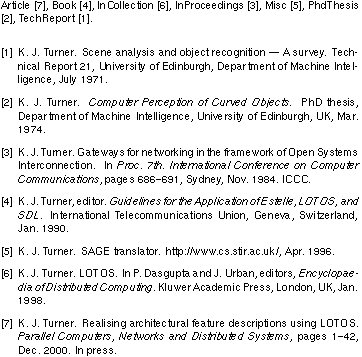
\includegraphics[width=0.7\linewidth]{showbst-abbrv.png}
						}
						\only<3>{
							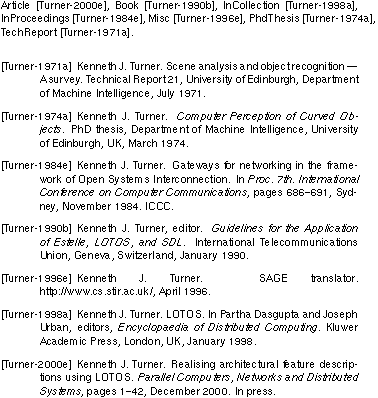
\includegraphics[width=0.7\linewidth]{showbst-abstract.png}
						}
					\end{center}
				\end{overlayarea}
		\end{columns}
	\end{frame}

	\begin{frame}{How generate bib files }
		\begin{columns}
			\column{.3\textwidth}
				\begin{overlayarea}{\textwidth}{\textheight}	
					\vspace{7em}
					\begin{block}{
							\only<1-2>{
								Bibfile Mendeley:
							}
							\only<3-4>{
								Bibfile Calibre:
							}
						}
						\only<2>{
									For articles
						}
						\only<4>{
									For Books.
						}
					\end{block}
				\end{overlayarea}	
			\column{.5\textwidth}
				\begin{overlayarea}{.5\textwidth}{\textheight}
					\vspace{7em}
					\only<2>{
								\href{run:MendeleyBibFile.mp4}{
								
\includegraphics[scale=0.25]{/home/saul/sauld@cimat.mx/Materias/Presentations/EnglishTalkNovember2014/logos/logoMendeley.jpg}%
							}
					}
					\only<4>{
								\href{run:CalibreBibFile.mp4}{
								
\includegraphics[scale=0.25]{/home/saul/sauld@cimat.mx/Materias/Presentations/EnglishTalkNovember2014/logos/logoCalibre.png}
							}
					}
				\end{overlayarea}
		\end{columns}
	\end{frame}

	\begin{frame}[fragile]{General Template }
		\begin{columns}
			\column{.3\textwidth}
				\begin{overlayarea}{\textwidth}{\textheight}	
					\vspace{3em}
					\begin{block}{Bib\TeX}
						\only<2>{
						Style (.bst)
 						}
						\only<3>{
						Database (.bib)
						}
					\end{block}
					\only<4>{
								\href{run:BibBSTWhere.mp4}{Bib\TeX}
							}
				\end{overlayarea}
			\column{.5\textwidth}
				\begin{overlayarea}{.5\textwidth}{\textheight}
						\vspace{1em}
						\begin{verbatim}
							\documentclass[11pt]{article}
							\usepackage{cite}
							\begin{document}
							    \title{My Article}
							    \author{Nobody Jr.}
							    \date{Today}
							    \maketitle
							
							    Blablabla \cite{Nobody06}.
							
							    \bibliographystyle{plain}
							    \bibliography{mybib}{}
							
							\end{document}
						\end{verbatim}
				\end{overlayarea}
		\end{columns}
	\end{frame}
	\subsection{Example 3: Generate a bib file with Mendeley}
	\subsection{Example 4: Generate a bib file whit Calibre}
	\section{Use Mendeley and Calibre with \LaTeX}
	\begin{frame}{Bibliography}
		\nocite{*}
		\printbibliography 
	\end{frame}
\end{document}